%!TEX TS-program = xelatex
\documentclass[]{friggeri-cv}
\usepackage{afterpage}
\usepackage{hyperref}
\usepackage{color}
\usepackage{xcolor}
\hypersetup{
    pdftitle={},
    pdfauthor={},
    pdfsubject={},
    pdfkeywords={},
    colorlinks=false,       % no lik border color
   allbordercolors=white    % white border color for all
}
\addbibresource{bibliography.bib}
\RequirePackage{xcolor}
\definecolor{pblue}{HTML}{0395DE}

\begin{document}
\header{James}{Knott}
      {Sr. DevOps Engineer}
      
% Fake text to add separator      
\fcolorbox{white}{gray}{\parbox{\dimexpr\textwidth-2\fboxsep-2\fboxrule}{%
.....
}}

% In the aside, each new line forces a line break
\begin{aside}
  \section{Available Work Locations}
    San Francisco, CA
    Chicago, IL
    New York City, NY
    Moscow, Russia
    Hong Kong, China
    Mexico
    ~
  \section{Telephone}
    (312) 420-5482
    

  \section{Mail}
    \href{mailto:devops@buildmystartup.io}{\textbf{devops@}\\buildmystartup.io}
    ~
  \section{Personal Projects}
    \href{http://www.buildmystartup.io}{buildmystartup.io}
  \href{http://www.weekendjobsearch.com}{weekendjobsearch.com}
  \href{http://www.devopsengineer.guru}{devopsengineer.guru}
    ~
  \section{Programming}
    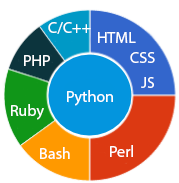
\includegraphics[scale=0.62]{img/programming_new.png}
    ~
  \section{Skill Level}
    \textbf{Linux}
\includegraphics[scale=0.40]{img/5stars.png}
    \textbf{AWS}
\includegraphics[scale=0.40]{img/4stars.png}
    \textbf{Python}
\includegraphics[scale=0.40]{img/4stars.png}
    \textbf{Chef}
\includegraphics[scale=0.40]{img/5stars.png}
    \textbf{Puppet}
\includegraphics[scale=0.40]{img/4stars.png}
    \textbf{Docker}
\includegraphics[scale=0.40]{img/4stars.png}
    \textbf{Jenkins}
\includegraphics[scale=0.40]{img/4stars.png}
    \textbf{Ansible}
\includegraphics[scale=0.40]{img/5stars.png}
    \textbf{Terraform}
\includegraphics[scale=0.40]{img/4stars.png}
    ~
  \section{My DevOps Experience}
    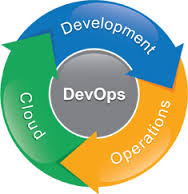
\includegraphics[scale=0.62]{img/second.jpg}
    ~
\end{aside}

\section{Experience}
\begin{entrylist}
\entry
    {03/17 - Now}
    {Sr. DevSecOps Engineer}
    { Here Technologies }
    {Design, Architect and Support multiple Docker Orchestrators, and Cloud Providers. AWS, Azure and Google. DC/OS, Mesosphere, Marathon, Kubernetes and AWS ECS. Toolchain and TechStack: Java, Ruby on Rails, Scala, AWS Elastic Beanstalk, ASG, VPC, S3, CloudFormation, EC2 Container Service(Docker),ElastiCache, Terraform, Packer, Ansible, Jenkins, Datadog, New Relic, MongoDB, RDS, Redis, Vagrant, Virtualbox, GitLab, Gerrit, OSX, Ubuntu, Centos, CoreOS ,Python, Bash, Shell. Consul, ETCD, Zookeeper, BackTrack, Kali, Nessus, Metasploit\\}
\entry
    {11/16 - 03/17}
    {Sr. DevOps Engineer}
    { Houseparty social network app }
    {Design, Architect, and Implemented new solutions to help company grow with expanding user base.           Build, maintain and support existing HA Clusters in AWS to support over 2 million concurrent users connecting from iPhone and Android mobile apps.     Toolchain and TechStack: Java, Ruby on Rails, Django, Flask, PHP, Scala, AWS Elastic Beanstalk, ASG, VPC, S3, CloudFormation, Kubernetes, EC2 Container Service(Docker),ElastiCache, Terraform, Packer, Ansible, Jenkins, Datadog, New Relic, MongoDB, Redis, Vagrant, Virtualbox, GitLab, OSX, Ubuntu, Centos ,Python, Bash, Shell.\\}
  \entry
    {07/14 - 02/17}
    {Sr. DevOps Engineer}
    {First Data Technologies }
    {Architect and Design DevOps Pipeline for external clients in AWS.           Migrated over 200 external clients from Bare metal, and Vmware environments in Private DataCenter to AWS. Designed Puppet and Chef solution for over 15,000 servers on site both Windows and Linux.     Toolchain and Techstack:Java, Ruby on Rails, Django, Flask, PHP, Scala, AWS (Elastic Beanstalk, ASG, VPC, S3, CloudFormation, EC2 Container Service(Docker),ElastiCache, Terraform, Packer, Ansible, Jenkins, Splunk, MySQL, MemcacheD, ELK Stack, Graylog, Vagrant, Virtualbox, GitLab, OSX, Ubuntu, Centos ,Python, Bash, Shell .\\}
  \entry
    {09/11 - 07/14}
    {Linux DevOps Engineer}
    {Mosaic}
    {Architected, Designed, Implemented and Supported main company virtual desktop solution using OpenStack, Redhat, NoMachine(Linux terminal services solution), OpenLDAP for centralized login. NSF shares for home folders, MySQL for logging user sessions, and all designed with HA and DR using loadbalancing and reverse proxy, across multiple datacenters.\\}
    \entry
    {02/10 - Now}
    {Technology Instructor and Personal Projects}
    {Hacker School}
    {Teach students DevOps, Full Stack Development and Open Source Solutions. Freelance Website Designer, Mobile Application Developer, DevOps Engineer. Current Open Source Project called Remote Command Center and is a solution for Roaming profiles for Linux. \\}
      \entry
    {1999/2010}
    { 1999 - 2002 Systems Admin (IT Services) 2002-2008 Network Architect II (Healthcare) ,2003 - 2005 Security Engineer, 2008 - 2010 Sr. Systems Engineer (HealthCare) }
    {}
    { \\}
\end{entrylist}




\begin{flushleft}
\emph{}
\end{flushleft}
\begin{flushright}
\emph{}
\end{flushright}

%%% This piece of code has been commented by Karol Kozioł due to biblatex errors. 
% 
%\printbibsection{article}{article in peer-reviewed journal}
%\begin{refsection}
%  \nocite{*}
%  \printbibliography[sorting=chronological, type=inproceedings, title={international peer-reviewed conferences/proceedings}, notkeyword={france}, heading=subbibliography]
%\end{refsection}
%\begin{refsection}
%  \nocite{*}
%  \printbibliography[sorting=chronological, type=inproceedings, title={local peer-reviewed conferences/proceedings}, keyword={france}, heading=subbibliography]
%\end{refsection}
%\printbibsection{misc}{other publications}
%\printbibsection{report}{research reports}

\end{document}
